\documentclass[a4paper,10pt]{article}
\usepackage[T1]{fontenc}
\usepackage[utf8]{inputenc}
\usepackage[frenchkw]{algorithm2e}
\usepackage[francais]{babel}
\usepackage{graphicx}
\usepackage{amsfonts}
\usepackage{amsmath}

%opening
\title{}
\author{}

\begin{document}

\maketitle

\begin{abstract}
%a la fin
\end{abstract}

\section{Qu'est ce qu'un système de recommandation?}

\subsection{Notre approche}
Le but de notre projet est de recommander un film à un utilisateur spécifique. 
Pour cela, nous devons savoir à quel point un utilisateur aime tel ou tel film pour lui recommander (ou pas). 
Il nous faudrait donc une sorte d'échelle d'affinité de l'utilisateur au film, ce qui parait pertinent est donc d'estimer une note qu'un utilisateur mettrait à un film s'il avait à le noter par exemple. 
Si cette note est au dessus d'un certain seuil, on lui recommandera (ou on recommandera le film ayant la meilleur note prédite par exemple). 
Notre approche du problème est donc de trouver un modèle mathématique permettant de trouver la note que mettrait un utilisateur à un film qu'il n'a pas vu. 
Cependant, sans aucunes connaissances des gouts l'utilisateur et des caractéristiques des films ceci est impossible. 
Il nous faut donc récuperer des données déjà existentes sur des utilisatuers et des films pour avoir une base et commencer à chercher une méthode.  
Nous avons donc récuperer des données.

\subsection{Première difficulté : les données}
\subsubsection{Extraction des données}
Le besoin d'avoir des données nous à guider vers une grande base de données appelé `` movielens '' qui est un site communautaire de recommandation de films où les utilisateurs du site notent des films de 0 à 5.  
Plusieurs jeux de données étaient disponibles et différé entre eux selon leur taille,  
Nous avons choisi de travailler avec une base de données de 670 utilisateurs (nu) et 9125 films (nf).  
On a donc extrait 2 fichiers : l’un contenant les 9125 films avec leurs titres et un numéro attribué ,  
l’autre avec les notes des utilisateurs qui avaient chacun un identifiants,  
le fichier était du type : identifiant de l’utilisateur, id du film qu’il a noté, note. 
Ces 2 fichiers étaient donc peu pratiques pour commencer à faire quelque chose avec,  
nous avons donc créer une fonction tableau\_des\_notes() qui permet de ranger toutes ces notes dans un tableau numpy nu*nf avec en lignes les utilisateurs,  
et en colonnes les films. Quand un utilisateur n’a pas vu un film donc qu’il ne l’a pas noté,  
on insère un `` Nan ''(Not a Number) qui est un `` symbole '' facile à traiter. On appellera ce tableau Y tout au long du projet. 
\subsubsection{Analyse des données}
Dans la logique des choses, notre tableau Y étant bien trop grand pour en tirer des conclusions 
juste à l’œil, nous avons créer des fonctions permettant de faire des sortes de statistiques sur nos données.
Nous avons crées quelques fonctions pour étudier nos données: l’une permettant de compter combien de films
chaque utilisateur a vu (cf nbre\_de\_films\_vu\_par\_utilisateur), et l’autre comptant combien de fois avait été noté chaque film 
(cf nbre\_de\_notes\_par\_film). De ces fonctions, nous avons pu tirer des graphiques nous montrant comment été répartis nos données.


Nous avons remarqué que la grande majorité des films possédaient entre 0 et 40 notes(Plus de 8000 sur 9000). 
Le nombre de notes le plus récurrents étant de 2 notes par film. Mais il y a tout de même quelques films qui ont été
beaucoup vu sachant que celui qui a le plus de note en a 339.

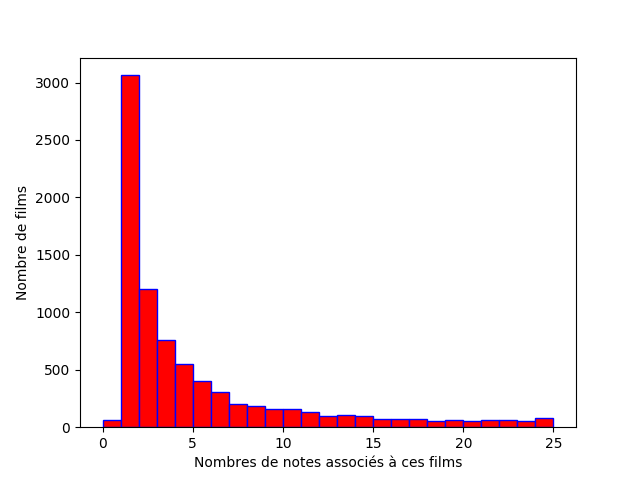
\includegraphics{hist2.png}

Dans l’autre sens,on remarque que en moyenne les utilisateurs ont noté 148 films, et la majorité est répartis entre blabla et babla films vus.

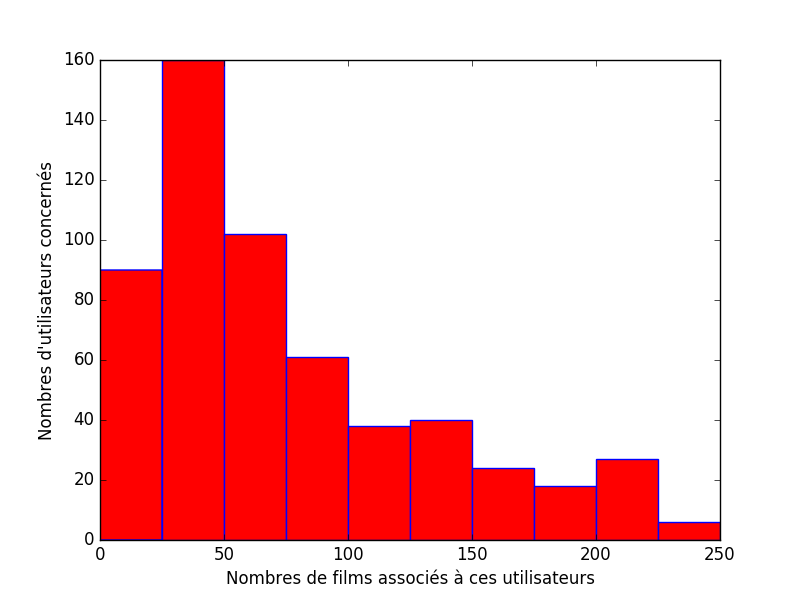
\includegraphics{hist1.png}

→ conclusion sur les données ce qu’on peut en tirer …
Notre tableau présente 98,4 \% de NaN. Cela nous fait donc plus de 6 millions de notes à prédire… Dans la prochaine partie,
nous verrons donc la méthode permettant de prédire toutes ces notes à partir de très peu de données c'est à dire notre tableau Y.


\section{Formalisation du problème d'optimisation y compris modélisation}

Nous nous posons maintenant la question comment nous y prendre pour prédire des notes ?
Notre seul ressource est la matrice Y non pleine, sur quel modèle s'appuyer pour la compléter ?
C'est ce que nous allons étudier dans cette partie.

\subsection{Factorisation}

Posons $Y_f$ la matrice Y complétée qui contient toutes les prédictions, exactes, des notes qui nous manquent. C'est la matrice à laquelle nous voulons aboutir, que nous devons deviner. Voici notre méthode.\\ 
 
Nous supposons que nous sommes capable de déterminer (et nous verrons que nous le sommes) à partir de Y deux matrices X et $\Theta$ telles que $\Theta X^T = Y_f$ avec $\Theta$ une matrice de dimension $n_u * n$ et X une matrice de dimension $n_f * n$. $n \in \mathbb{N}^*$ est quelconque, nous verrons par la suite que nous pouvons le fixer comme bon nous semble. 
Autre chose, nous ne voulons pas déterminer deux matrices $\Theta$ et X quelconques qui vérifient les propriétés énoncées ci-dessus mais deux matrices particulières : $\Theta$ représentant les profils de chaque utilisateur et X les caractéristiques des films. Nous allons éclairer ce point tout de suite par des explications plus précises.\\ 
 
Supposons pour ces explications que nous avons déjà déterminé $\Theta$ et X avec $n \in \mathbb{N}^*$ que nous avons choisi. Ce dernier est en fait un nombre de caractéristiques quelconques qui peuvent bien décrire nos films. Par exemple, si nous pensons que nos films peuvent être décris efficacement par 10 caractéristiques, nous choisissons $n = 10$. 
Les n sont déterminées en même temps que $\Theta$ et X mais elles nous sont inconnues, une caractéristique peut être un taux d'action, le taux de blondeur des cheveux de l'actrice principale, etc. Pour l'instant admettons seulement que ces n caractéristiques existent puis nous verrons comment elles sont déterminées dans une autre partie. 



\subsection{Fonction cout}
%toujours antho
\subsubsection{Pourquoi on cherche a minimiser}
\section{Implémentation algo}
%guillaume
\subsection{descente du gradient en general optimisation}
Nous utilisons un algorithme appelé descente du gradient pour minimiser J. Pour illustrer cet algorithme nous allons l'appliquer 
a une fonction $f$ qui depend de deux variables.%J'aimerai bien mettre la n otation pour une fonction ici
 On a $df = \frac{\partial f}{\partial x_{1}}d x_{1} + \frac{\partial f}{\partial x_{2}}dx_{2}$. En faisant l'approximation
 $\Delta f = \frac{\partial f}{\partial x_{1}}\Delta  x_{1} + \frac{\partial f}{\partial x_{2}}\Delta x_{2}$ on se rend compte
 que en posant $\Delta x_{1} = -\alpha \frac{\partial f}{\partial x_{1}}$
 et $\Delta x_{2} = -\alpha \frac{\partial f}{\partial x_{2}}$ avec $\alpha \in \Re^{+}$
 on obtient $\Delta f = -\alpha \frac{\partial f}{\partial x_{1}}^{2} - \alpha \frac{\partial f}{\partial x_{2}}^{2} < 0$. Ainsi dans
 les limites de l'approximation faite au dessus on a un moyen de minimiser E.
L'idée dérriere la descente du gradient 
est de descendre la pente de al fonction donc le gradient que nous nommons $\nabla_{x}$ pour le gradiant de la fonction par rapport 
a $x$. Une explication plus détaillé de la notation est donné en annexe.  
 
\begin{algorithm}[H]
 \Donnees{a mettre} 
 \Res{un nouveau x} 
 initialization\;
 \PourTous{j $\in$ \{1, 2, ..., nf\}}{
  Affecter à $x_{j}$ la valeur $x_{j}-\alpha \nabla_{x_{j}}J(x, \Theta)$\;
 }
 \caption{Descente du gradient}
\end{algorithm}
%je sais que c'est trop court et pas assez bien posé mais il faut commencer quelque part
On prouve en \ref{P1} que $ \nabla_{x_{j}}J(x, \Theta) = \nabla_{x_{j}^T}\frac{1}{2}\Vert\tilde{\theta}x_{j}^{T}-\tilde{y}_{.,j}\Vert^{2}$
puis en \ref{P2} on prouve que $[\nabla_{x} \frac{1}{2}||Ax - b||^{2}_{2}]_{j} = [A^{T}(Ax - b)]_{j}$ ce qui nous permet de dire
que $ \nabla_{x_{j}}J(x, \Theta) =  \tilde{\theta}^{T}(\tilde{\theta}x_{j}^{T}-\tilde{y}_{.,j})$. Ces divers calculs nous permettent
de representer une étape du gradient comme une série de produits de matrices. Au début nous devions calculer le résultat terme a terme. Cette
facon de faire était trés lente et passer a une représentation matricielle nous a permis de grandement accelerer les etapes de la descente d gradient.
\subsubsection{ecrire algo puis dire comment on a fait au début}
\section{Mise en application de l'algorithme}
\subsection{Familiarisation avec problème plus simple}
Dans la première partie de notre projet, nous avons décidé de simplifier notre problème en extrayant un tableau de données 
plein c'est à dire un tableau où tous les films ont été notés par tous les utilisateurs. 
A partir de ce tableau, nous pouvons donc enlever une note et essayer de la prédire. Ainsi, nous pouvons voir nos erreurs facilement.
Notre première difficulté a été d'extraire ce tableau plein. Pour cela, l'étude des données faite en amont nous a beaucoup aidé: pour extraire ce tableau ``plein''
nous avons crées une fonction (cf annexe) sélectionnant les films les plus vus puis les utilisateurs qui ont vues tous ces films. On a donc obtenus un
tableau plein 10*10 (10films pour 10 utilisateurs) ce qui nous a permis d'appliquer la descente du gradient rapidement sur notre petit tableau de données. Ainsi,
nous avons pu appliquer notre première descente du gradient.
\subsection{yassine}
\subsubsection{taux d'erreur}
\subsubsection{influence des parametres}
\subsection{limites de notre approche}
%yassine
\subsubsection{Est-ce qu'on arrive a reccomander un film a un utilisateur}
%guillaume
Au final une question intéressante est est-ce que le modèle arrivera d'une maniére efficace a predire les notes a un nouvel utilisateur. Pour faire cela nous avons
choisi de ne pas recalculer $X$ et $\Theta$ pour chaque nouvel utilisateur a la place nous supposons que l'ajout d'un utlilisateur ne va pas modifier
les caractéristiques d'un film. Il nous suffit donc de calculer $\theta$ pour l'utlisateur seulement. Ceci peut se faire trés rapidement comme notre $\Theta$ ne
consiste que du vecteur de préferences de l'utilisateur. A partir de ces nouvels donnés il nous suffit de calculer Y pour trouver la note la plus élevée et la reccomander
a l'utilisateur. Toutefois l'erreur sur la prediction des notes nous laisse penser que ce film ne serzit pas probablement le meilleur film
pour cette utilisateur car le hasard aurait bien pu faire que le meilleur film ait une note plus basse de 1 point ce qui suffi a lui faire perdre la premiére place.
\section{conclusion}
%1 page

\subsection{perspectives}
%guillame
\appendix
\section{Preuves}
\subsection{}
\label{P1}
$\nabla_{x_{j}^T} J(\theta, X)=
\begin{pmatrix}
\displaystyle\frac{\partial \displaystyle\sum_{k=1}^{nf}\frac{1}{2}\Vert\tilde{\theta}x_{k}^{T}-\tilde{y}_{.,k}\Vert^{2}}{\partial x_{j,1}^{T}}\\
\displaystyle\frac{\partial \displaystyle\sum_{k=1}^{nf}\frac{1}{2}\Vert\tilde{\theta}x_{k}^{T}-\tilde{y}_{.,k}\Vert^{2}}{\partial x_{j,2}^{T}}\\
\vdots\\
\displaystyle\frac{\partial \displaystyle\sum_{k=1}^{nf}\frac{1}{2}\Vert\tilde{\theta}x_{k}^{T}-\tilde{y}_{.,k}\Vert^{2}}{\partial x_{j,n}^{T}}
\end{pmatrix}
=
\begin{pmatrix}
\displaystyle\sum_{k=1}^{nf}
\frac{1}{2}\frac{\partial\Vert\tilde{\theta}x_{k}^{T}-\tilde{y}_{.,k}\Vert^{2}}{\partial x_{j,1}^{T}}\\
\displaystyle\sum_{k=1}^{nf}
\frac{1}{2}\frac{\partial\Vert\tilde{\theta}x_{k}^{T}-\tilde{y}_{.,k}\Vert^{2}}{\partial x_{j,2}^{T}}\\
\vdots\\
\displaystyle\sum_{k=1}^{nf}
\frac{1}{2}\frac{\partial\Vert\tilde{\theta}x_{k}^{T}-\tilde{y}_{.,k}\Vert^{2}}{\partial x_{j,n}^{T}}
\end{pmatrix}$\\
$
=
\begin{pmatrix}
\displaystyle
\frac{1}{2}\frac{\partial\Vert\tilde{\theta}x_{j}^{T}-\tilde{y}_{.,j}\Vert^{2}}{\partial x_{j,1}^{T}}\\
\displaystyle
\frac{1}{2}\frac{\partial\Vert\tilde{\theta}x_{j}^{T}-\tilde{y}_{.,j}\Vert^{2}}{\partial x_{j,2}^{T}}\\
\vdots\\
\displaystyle
\frac{1}{2}\frac{\partial\Vert\tilde{\theta}x_{j}^{T}-\tilde{y}_{.,j}\Vert^{2}}{\partial x_{j,n}^{T}}
\end{pmatrix}
=
\displaystyle
\nabla_{x_{j}^T}\frac{1}{2}\Vert\tilde{\theta}x_{j}^{T}-\tilde{y}_{.,j}\Vert^{2}
$
\subsection{}
\label{P2}
\begin{align*}
[\nabla_{x} \frac{1}{2}||Ax - b||^{2}_{2}]_{j} &= [\nabla_{x} \frac{1}{2}(\sum^{n}_{i = 1} (\sum^{p}_{k = 1} A_{i, k}x_{k})^{2} - 2b_{i}(\sum^{p}_{k = 1} A_{i, k}x_{k}) + b_{i}^{2})]_{j}\\
[\nabla_{x} \frac{1}{2}||Ax - b||^{2}_{2}]_{j} &= \frac{\partial\frac{1}{2}(\sum^{n}_{i = 1} (\sum^{p}_{k = 1} A_{i, k}x_{k})^{2} - 2b_{i}(\sum^{p}_{k = 1} A_{i, k}x_{k}) + b_{i}^{2})}{\partial x_{j}}\\
[\nabla_{x} \frac{1}{2}||Ax - b||^{2}_{2}]_{j} &= \frac{1}{2}(\sum^{n}_{i = 1} 2(\sum^{p}_{k = 1} A_{i, k}x_{k})A_{i, j} - 2b_{i} A_{i, j})\\
[\nabla_{x} \frac{1}{2}||Ax - b||^{2}_{2}]_{j} &= (\sum^{n}_{i = 1} (\sum^{p}_{k = 1} A_{i, k}x_{k})A_{i, j} - b_{i} A_{i, j})\\
[\nabla_{x} \frac{1}{2}||Ax - b||^{2}_{2}]_{j} &= (\sum^{n}_{i = 1} A_{i, j}(\sum^{p}_{k = 1} A_{i, k}x_{k}) - b_{i} )\\
[\nabla_{x} \frac{1}{2}||Ax - b||^{2}_{2}]_{j} &= \sum^{n}_{i = 1} A^{T}_{j, i}[Ax - b]_{i}\\
[\nabla_{x} \frac{1}{2}||Ax - b||^{2}_{2}]_{j} &= [A^{T}(Ax - b)]_{j}
\end{align*}
\end{document}